\chapter{Introduction}
\vspace{-1.4em}

%\begin{figure}[ht]
 %\begin{center}
%trim option's parameter order: left bottom right top, remove square brackets for no trim
 %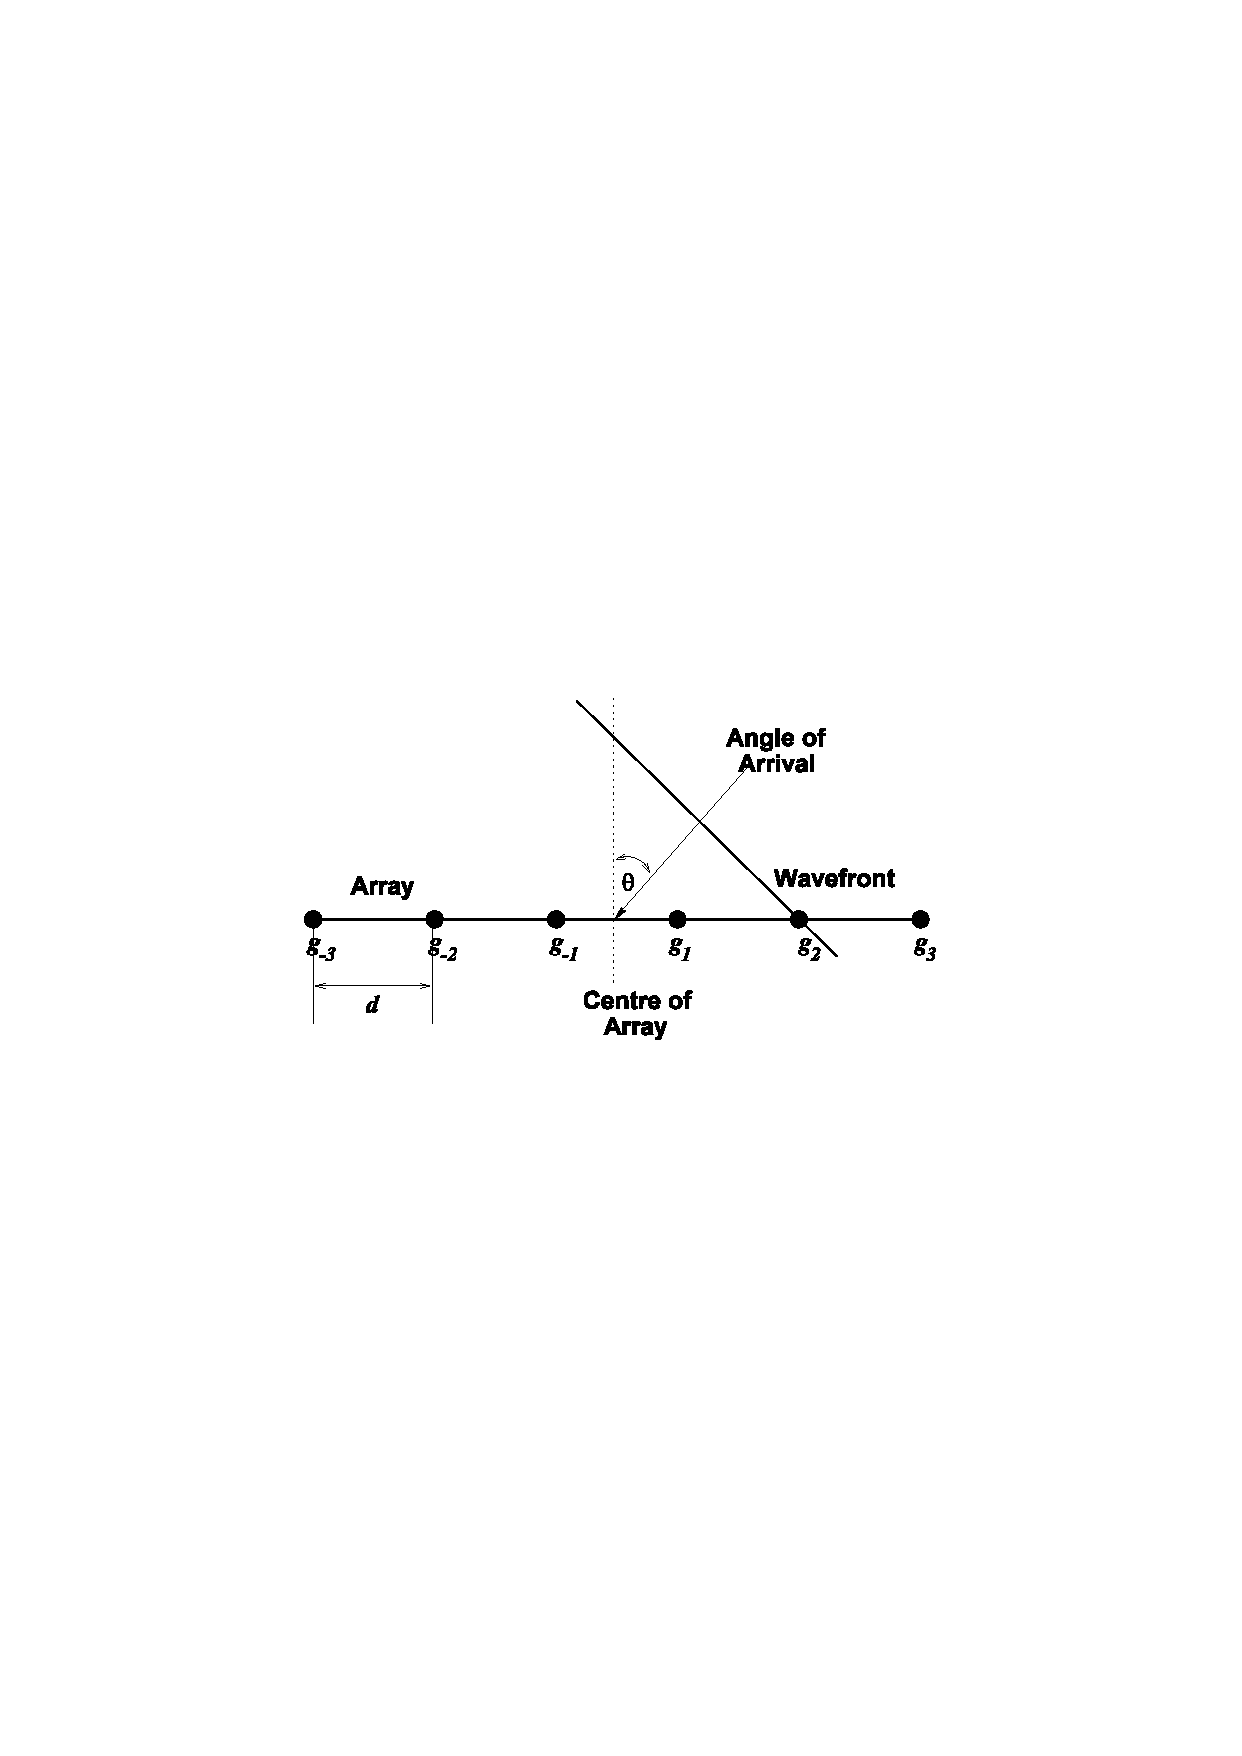
\includegraphics[trim = 50.5mm 100.2mm 50.8mm 117.3mm, clip, width=10cm]{images/antenna_array}
 %\end{center} 
 %\vspace{-1cm}
 %\caption{A uniform linear antenna array showing the angle of arrival of an incoming planar wavefront.}
% \label{fig:antenna_array}
%\end{figure}

\section{Direct Digital Synthesiser based VHF Tranceiver}

The DDS chosen is AD9854 from Analog Devices

The board used in specific is the 



\section{Current application of AD9854 DDS}




\section{Approach - Raspberry Pi driven DDS}

The aim of this project is to design of a low-cost radio transceiver of 70MHz, using the AD9854 Direct Digital Synthesiser and Raspberry Pi. The programming of synced signal will be done in C language. The transmission of samples is uniform in time.
The I and Q synthesizer function, or the RF signal, used for this research topic is: 

\begin{equation}
I(t)\cos(\omega t)+Q(t)\sin(\omega t)
\end{equation}

For signal receiver, the version 3 RTL-SDR radio receiver dongle will be used, which samples a radio frequency signal from 50 MHz to 1700MHz and outputs interleaved 8-bit IQ samples at s symbol rate up to 2.4Msps.




\section{Project scope and requirement}
Project Scope: The work performed to deliver a product, service or result with the specified features and functions. 
Requirement: A condition or capability that is required to be present in a product, service or result to satisfy a contract or other formally imposed specification.
This project is focused on implementing a transceiver with the mentioned components using knowledge on how an IQ modulator works and how to program the synced signals in C. 
There was no previous attempt on using AD9854 DDS in combination with the Raspberry Pi to implement a transceiver, hence this might be the biggest challenge. The feasibility of this design is to be analysed during the progress. There may be incompatibility between Raspberry Pi and AD9854 and this will be determined whether an issue in primary stages.



\section{Project Objective}
The project objective is to learn how an IQ modulator works and how to program synthesised signals in C programming language.
Furthermore, the cost of the design is to be kept low.



\section{Organization of thesis}

The aim of this thesis is to present the 
Chapter 1 presents the purpose of building a low-cost VHF transceiver, and the current 
Chapter 2
Chapter 3
Chapter 4






